\begin{comment}
\[
    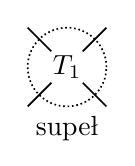
\begin{tikzpicture}[baseline=-0.65ex, scale=0.1]
    \useasboundingbox (-5, -9) rectangle (5, 5);
        \draw[semithick] (-2, -2) to (-5,-5);
        \draw[semithick] (2, 2) to (5,5);
        \draw[semithick] (2, -2) to (5,-5);
        \draw[semithick] (-2, 2) to (-5,5);        %
        \draw[semithick, densely dotted] (-0, 0) circle (5);
        \node at (0, 0) {$T_1$};
        \node [below] at (0, -5) {supeł};
    \end{tikzpicture}
    \quad \quad
    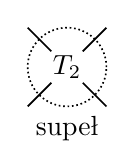
\begin{tikzpicture}[baseline=-0.65ex, scale=0.1]
    \useasboundingbox (-5, -9) rectangle (5, 5);
        \draw[semithick] (-2, -2) to (-5,-5);
        \draw[semithick] (2, 2) to (5,5);
        \draw[semithick] (2, -2) to (5,-5);
        \draw[semithick] (-2, 2) to (-5,5);        %
        \draw[semithick, densely dotted] (-0, 0) circle (5);
        \node at (0, 0) {$T_2$};
        \node [below] at (0, -5) {supeł};
    \end{tikzpicture}
    \quad \quad
    % \begin{tikzpicture}[baseline=-0.65ex, scale=0.1]
    % \useasboundingbox (-15, -9) rectangle (15, 5);
    %     \draw[semithick] (-12, -2) to (-15,-5);
    %     \draw[semithick] (-12, 2) to (-15,5);        %
    %     \draw[semithick, densely dotted] (-10, 0) circle (5);
    %     \node at (-10, 0) {$T_1$};
    %     \draw[semithick] (12, -2) to (15,-5);
    %     \draw[semithick] (12, 2) to (15,5);        %
    %     \draw[semithick, densely dotted] (10, 0) circle (5);
    %     \node at (10, 0) {$T_2$};
    %     \draw[semithick] (-8, 2) [in=135, out=45] to (8, 2);
    %     \draw[semithick] (-8, -2) [in=-135, out=-45] to (8, -2);
    %     \node [below] at (0, -5) {produkt};
    % \end{tikzpicture}
    % \quad \quad
    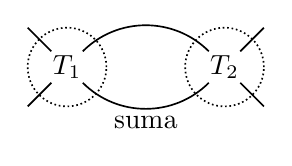
\begin{tikzpicture}[baseline=-0.65ex, scale=0.1]
    \useasboundingbox (-15, -9) rectangle (15, 5);
        \draw[semithick] (-12, -2) to (-15,-5);
        \draw[semithick] (-12, 2) to (-15,5);        %
        \draw[semithick, densely dotted] (-10, 0) circle (5);
        \node at (-10, 0) {$T_1$};
        \draw[semithick] (12, -2) to (15,-5);
        \draw[semithick] (12, 2) to (15,5);        %
        \draw[semithick, densely dotted] (10, 0) circle (5);
        \node at (10, 0) {$T_2$};
        \draw[semithick] (-8, 2) [in=135, out=45] to (8, 2);
        \draw[semithick] (-8, -2) [in=-135, out=-45] to (8, -2);
        \node [below] at (0, -5) {suma};
    \end{tikzpicture}
\]
\end{comment}
